\subsection{Caso d'uso UC1: Interazione con una presentazione}
\begin{figure}[h] 
	\centering 
	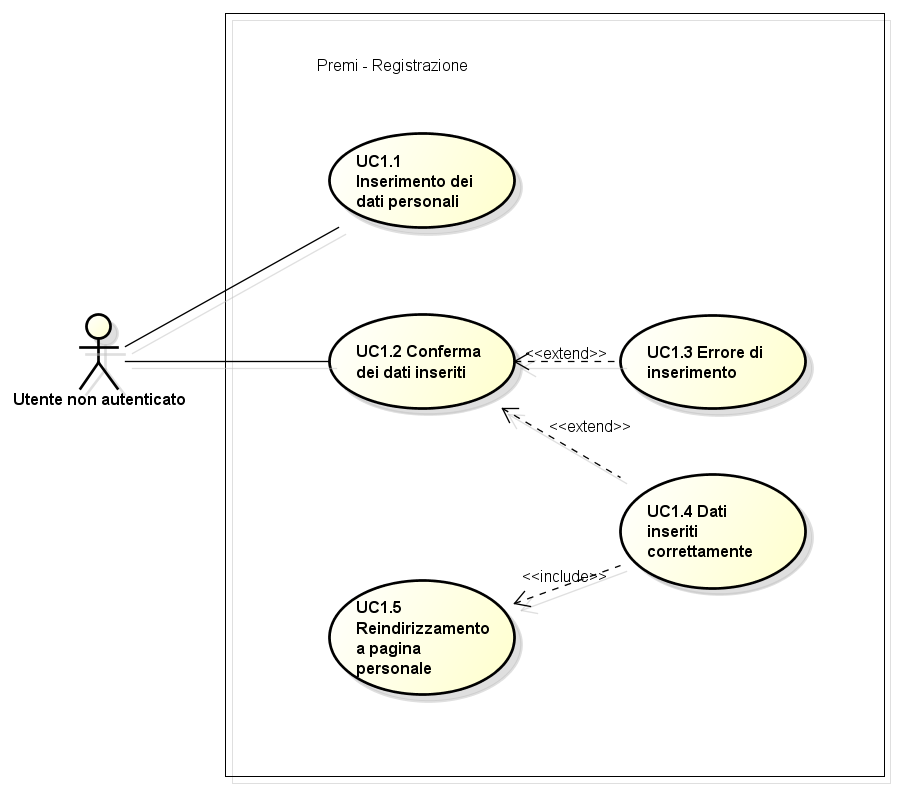
\includegraphics[scale=0.45] {img/UC1.png} 
	\caption{UC1 - Interazione con una presentazione} 
\end{figure}

\begin{itemize}
	\item \textbf{Attori:} Visualizzatore;
	\item \textbf{Scopo e descrizione:} L'utente vuole visualizzare una presentazione: cerca la presentazione che gli interessa, ne fa il download e una volta salvata può visualizzarla in modalità offline. Inoltre può anche scegliere di stampare la presentazione scaricata;
	\item \textbf{Precondizione:} L'utente visualizzatore è pronto a cercare una presentazione;
	\item \textbf{Flusso degli eventi:}
	\begin{enumerate}
		\item Il visualizzatore cerca una presentazione [UC1.1];
		\item Il visualizzatore esegue il download della presentazione [UC1.2];
		\item Il visualizzatore visiona la presentazione scaricata [UC1.3];
		\item Il visualizzatore può scegliere di stampare la presentazione [UC1.4].
	\end{enumerate}
	\item \textbf{Postcondizione:} Il visualizzatore ha ottenuto le informazioni che voleva.
\end{itemize}

\subsection{Caso d'uso UC1.1: Cercare una presentazione}
\begin{itemize}
	\item \textbf{Attori:} Visualizzatore;
	\item \textbf{Scopo e descrizione:} L'utente cerca la presentazione che sta cercando tra quelle disponibili;
	\item \textbf{Precondizione:} Il sistema è in attesa che l'utente cerchi una presentazione;
	\item \textbf{Postcondizione:} Il sistema mostra il risultato della ricerca dell'utente.
\end{itemize}

\subsection{Caso d'uso UC1.2: Download di una presentazione}
\begin{itemize}
\item \textbf{Attori:} Visualizzatore;
\item \textbf{Scopo e descrizione:} Una volta trovata la presentazione che gli interessa, il visualizzatore esegue il download della presentazione;
\item \textbf{Precondizione:} Il sistema è in attesa che l'utente esegua il download;
\item \textbf{Postcondizione:} Il sistema ha permesso al visualizzatore di scaricare e salvare la presentazione.
\end{itemize}

\subsection{Caso d'uso UC1.3: Visualizzare una presentazione}
\begin{itemize}
\item \textbf{Attori:} Visualizzatore;
\item \textbf{Scopo e descrizione:} L'utente apre la presentazione precedentemente scaricata e può visualizzarla in modalità offline secondo le sue preferenze;
\item \textbf{Precondizione:} Il sistema è in attesa che l'utente crei una casella di testo;
\item \textbf{Postcondizione:} Il sistema ha creato la casella di testo.
\end{itemize}

\subsection{Caso d'uso UC1.4: Stampare una presentazione}
\begin{itemize}
	\item \textbf{Attori:} Visualizzatore;
	\item \textbf{Scopo e descrizione:} L'utente una volta scaricata la presentazione, può decidere di stamparla;
	\item \textbf{Precondizione:} Il sistema è in attesa che l'utente scelga la funzione di stampa;
	\item \textbf{Postcondizione:} Il sistema avviato la procedura di stampa.
\end{itemize}

\newpage